\documentclass{cmn}

\begin{document}
  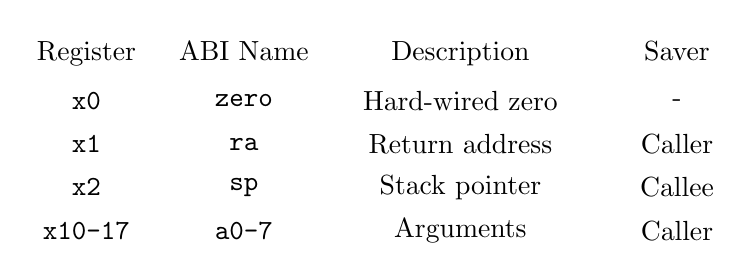
\begin{tikzpicture}
    \node at (0,0) {Register\vphantom{\strut}};
    \node at (20mm,0) {ABI Name\vphantom{\strut}};
    \node at (47.5mm,0) {Description\vphantom{\strut}};
    \node at (75mm,0) {Saver\vphantom{\strut}};

    \foreach \i/\t/\u/\v/\w in {1/x0/zero/Hard-wired zero/-,2/x1/ra/Return address/Caller,3/x2/sp/Stack pointer/Callee,4/x10-17/a0-7/Arguments/Caller} {
      \node at (0,-0.5mm-\i*5.5mm) {\texttt{\t}};
      \node at (20mm,-0.5mm-\i*5.5mm) {\texttt{\u}};
      \node at (47.5mm,-0.5mm-\i*5.5mm) {\v};
      \node at (75mm,-0.5mm-\i*5.5mm) {\w};
    }
  \end{tikzpicture}
\end{document}
